\documentclass[11pt]{article}
\usepackage[a4paper, margin=2.5cm]{geometry}  % 页边距
\usepackage{graphicx}
\usepackage{fancyhdr}
\usepackage{xcolor}
\usepackage{sectsty}
\usepackage{lipsum}
\usepackage{times} % 使用Times New Roman
% 页眉页脚
\pagestyle{fancy}
\fancyhf{}
\fancyhead[L]{\textcolor{gray}{\textit{\fontsize{10}{12}\selectfont CIV5886 - Infrastructure Geomechanics\\Assignment 2}}}
\fancyhead[R]{}
\fancyfoot[R]{Page \thepage\ of 8}
\renewcommand{\headrulewidth}{0pt}
\renewcommand{\footrulewidth}{0pt}
% 自定义标题格式
\sectionfont{\normalfont\bfseries\scshape\large}
\subsectionfont{\normalfont\bfseries\itshape\normalsize}
\newcommand{\sectiontitle}[1]{\noindent\textbf{\MakeUppercase{#1}}}
\newcommand{\firstletter}[1]{\textbf{\fontsize{14}{17}\selectfont #1}}
% 表格
\usepackage{booktabs}
\usepackage{multirow}
\usepackage{array}
% 链接
\usepackage[colorlinks=true, linkcolor=blue, urlcolor=blue]{hyperref}
% 引用link
\usepackage{hyperref}
% 此处偷懒,直接定义参考文献
\usepackage[english]{babel}
\usepackage[style=apa, backend=biber]{biblatex}
\DeclareLanguageMapping{english}{english-apa}
\addbibresource{references.bib}
\begin{filecontents}{references.bib}
@article{bib1,
  author    = {Ye Bai},
  title     = {Discussion on Engineering Geological Conditions and Construction Problems of the Yin-Hong-Ji-Shi Tunnel},
  journal   = {Groundwater},
  volume    = {36},
  number    = {05},
  pages     = {180--181},
  year      = {2014},
   note={{\color{blue}
  \href{https://kns.cnki.net/kcms2/article/abstract?v=9CXCstbk-tuXMdvgi_IKuYShNNRDEDkN82mz6ZaBEvkyNQ1Dz1KPgxDfVOqUDD_dFtc5093puSnNEsslOMJ_tP0259WHLAYqDx2n5b66bHpAFhHvwpR5DSvcrRK9tHR8raq-Ldb3vLJ0dA0NgMTbZA==&uniplatform=NZKPT&language=CHS}{URL}}}
}
@mastersthesis{bib2,
  author    = {Qinsheng Gao},
  title     = {Research and Application of Construction Techniques for the Yin-Hong-Ji-Shi Tunnel},
  school    = {Northwest A\&F University},
  year      = {2008},
   note={{\color{blue}
  \href{https://kns.cnki.net/kcms2/article/abstract?v=9CXCstbk-ttsYM4bCpaWFkpk6FMM6c2IW-W34OZ2Rkc6kOwXbtPmYHwF4_CT5eB1-ISkESzAy9Do48plmk-fS_fobzyTV2_gAEy1hUTtM6gWZFVonrjl3olsQuFZA05y0fKzh3aDtPDpDuSb_Yz-Vg==}{URL}}}
}
@article{bib3,
  author    = {Yi Guo},
  title     = {Understanding Construction of Unfavorable Geological Sections in the Yin-Hong-Ji-Shi Water Diversion Tunnel},
  journal   = {Shaanxi Water Resources},
  number    = {01},
  pages     = {75--76},
  year      = {2013},
  note={{\color{blue}
  \href{https://kns.cnki.net/kcms2/article/abstract?v=9CXCstbk-tuPJfJxr_vlHefRWfLIq9WBLsV7QknSvvDONJKvBTuPtcgnFVbw9Xs1tTYgIYUx5i97nu904LldVv_u2pPtzg5J4qxaiSJBu791xBIBS10XLJmPLC9Ro-Zl9gqmB6CSRBY=}{URL}}}
}
@article{bib4,
  author    = {Jiang Lei and Weizhong Chen and Fanfan Li and Hongdan Yu and Yongshang Ma and Huadong Xie and Fugang Wang},
  title     = {Study on Mechanical Characteristics of Surrounding Rock in the Yin-Hong-Ji-Shi Water Diversion Tunnel},
  journal   = {Rock and Soil Mechanics},
  volume    = {40},
  number    = {09},
  pages     = {3435--3446},
  year      = {2019},
  note={{\color{blue}
  \href{https://kns.cnki.net/kcms2/article/abstract?v=9CXCstbk-tsVA-jBfLdYBVKSlL2mI6ybg36z8Jmy5O_fNn-bWa_wDg8aKMpkqKXeaf4U438q-wAcKmLIebRWWaAibZ3J61ZVRpI0WDd6Q7PMfX5tIopYbmDWLKHyYm8SAZdlTeJDzlE=&uniplatform=NZKPT&language=CHS}{URL}}}
}
@article{bib5,
  author    = {Yongguo Ma},
  title     = {Construction of Waterproofing and Drainage in the Long Tunnel of the Yin-Hong-Ji-Shi Project},
  journal   = {Groundwater},
  volume    = {31},
  number    = {06},
  pages     = {161--163},
  year      = {2009},
  note={{\color{blue}
  \href{https://kns.cnki.net/kcms2/article/abstract?v=9CXCstbk-tv5c-D8qFKoU3YZcOHEaXKwkcyTASowfi4gU-fBNaqF1I--D0mu6QbincxWBPmX5UwULLSCqEUWenKip1O5LWxm6A8OJxoBHlJHKShE_7AtOQ2nqNziiLIcGNSUcLVLxTI=}{URL}}}
}
@article{bib6,
  author    = {Hai Wang},
  title     = {Discussion on the Initial Support Deformation Treatment in the Yin-Hong-Ji-Shi Tunnel},
  journal   = {Shaanxi Water Resources},
  number    = {04},
  pages     = {96--97},
  year      = {2012},
    note={{\color{blue}
  \href{https://kns.cnki.net/kcms2/article/abstract?v=9CXCstbk-ttLHzSjks_B1z7FU-EmWD3HT9wcZ_d9vLWeuPjq1gooSKTmAhc1SUQTDC5Qy1uCTDwGcBCb3Rr-nQZ4yB64n615Z4xMheN7e83lce2FyEiD_seMjGnSxsjZmurqH3qPUR0=}{URL}}}
}
@article{bib7,
  author    = {Haiqiang Xu},
  title     = {Design and Construction Techniques of TBM Equipment Modification and Chamber Expansion in the Yin-Hong-Ji-Shi Project},
  journal   = {Journal of Yan'an Vocational and Technical Institute},
  volume    = {26},
  number    = {01},
  pages     = {108--109},
  year      = {2012},
      note={{\color{blue}
  \href{https://kns.cnki.net/kcms2/article/abstract?v=9CXCstbk-tunNYhVP7pN6DoGZb_n8IE28W_dc28GCwsl3HfSHwm7oc58HqOO5iFL9uqDf3-Oo79JXs3IXEns_jL95dx8DCERVBnIV1RYcNLR9Wh8D2mjMs5m8uKfG7kEEDH5WDM5K0M=}{URL}}}
}
@conference{bib8,
  author    = {Minxian Zhang and Xiaohui Xu},
  title     = {Selection of Overall Layout Scheme and Key Technical Issues for the Yin-Hong-Ji-Shi Project},
  booktitle = {Conference on Technology Exchange in Water Transfer Engineering},
  location  = {Shenyang, Liaoning, China},
  year      = {2009}
}
\end{filecontents}

\begin{document}

% 题目
\begin{center}
{\LARGE \textbf{Analysis of Geotechnical Issues During Tunnel Construction}}\\[2ex]
{\LARGE \textbf{and Comparison of Construction Methods: A Case Study of}}\\[2ex]
{\LARGE \textbf{ Yin Hong Ji Shi Tunnel}}\\[2ex]
{\large Shengming Luo, Zilong Zhu, Xuehao Yin, Dongyi Li}\\[1ex]
{\large Discipline Coordinator: Dr. Yangyang Li}
\end{center}

% 第一部分
\section*{\sectiontitle{\firstletter{1} \hspace{0.1cm} \firstletter{I}ntroduction}}

\subsection*{1.1 Background}
Shaanxi province is one of the provinces with severely poor water resources in China, southern Shaanxi is relatively rich, and Guanzhong is a serious water shortage of resources. The ecological problems brought about by the water environment pollution of the Weihe River are very prominent. The lack of water resources has become a main constraint in Shaanxi province. The fundamental way to solve the problem of resource water shortage can only be to divert water from other basins.

\subsection*{1.2 Project Overview}
The Hongin Water Diversion Project, located in Taibai County, Baoji City, Shaanxi Province, is a significant cross-basin water diversion effort. This project transfers water from the Hongyan River, a tributary of the Hanjiang River, to the Stone River, a tributary on the south bank of the Weihe River. The water is diverted through a tunnel that passes through the Qinling Mountains \parencite{bib3}.

The total length of the tunnel is 19.76km, which is the longest single tunnel of water transmission tunnel in Shanxi province \parencite{bib6}. The buried depth of the tunnel is large, generally 150-300m. The lithology of the strata passing through the cave line is complex, and the faults converge centrally, so there may be some problems such as slight rock burst and surrounding rock creep in the construction.

The hongjiishi water diversion project is to transfer the water of the Han River into the Stone River, a tributary of the south bank of the Weihe River, through the tunnel of 19.76km through the Qinling Mountains \parencite{bib7}. The project revenue area is the four urban areas of Xi'an, Xianyang, Yangling and Baoji, which will provide production and living water for the urban area, and take into account the ecological water of the Weihe River. The construction of the project will play an important role in alleviating the water supply contradiction in the central and western Guanzhong cities and optimizing the allocation of water resources in the Weihe River basin. Therefore, carrying out the research of this topic can save the project cost, shorten the construction period, and achieve greater economic and social benefits.

\subsection*{1.3 Geological Overview}
The schematic diagram of the construction segmentation around the main tunnel excavation is shown in Fig.~\ref{fig1}. The entrance of the tunnel is located in Guanshan Village, 8km southwest of Taibai County, and the exit of the tunnel is located in Dujiazhuang Village, Taochuan Town, 12km east of Taibai County. The Hongyan River flows through more than 40 kilometers long natural river of Shishi River and enters the completed Shitouhe Reservoir located in Xiyu Guan Town, Mei County, Baoji City.

\begin{figure}[h]
\centering
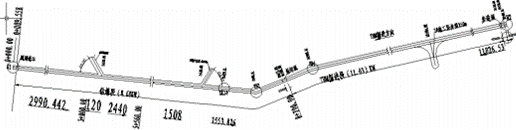
\includegraphics[width=0.9\textwidth]{mychart/22.png}
\caption{Sketch of construction subsection around main tunnel excavation \parencite{bib2}}\label{fig1}
\end{figure}

The inlet bottom elevation of the water conveyance tunnel is 1468.49m, and the outlet bottom elevation is 1446.29m. It is a pressureless free-flow water conveyance system with a longitudinal slope of 1/890 and a roughness coefficient of 0.014.

There are a total of 12 fractures related to the water diversion tunnel, especially fractures F1, F2, F5, F6, F12, F21, and others. These six fractures have the greatest impact and are concentrated in the area of the small reservoir. They intersect with each other, resulting in intense rock fragmentation. The geological conditions of the project are poor, which is unfavorable for the stability of the tunnel.

The geological formation that the tunnel passes through is primarily composed of Middle Proterozoic Qinling Group metamorphic rocks. The main rock types include biotite gneiss, schist, amphibolite, mica schist, quartz schist, and marble \parencite{bib8}. Within this formation, there are also Yanshanian granite intrusions, including gneissic biotite granite and a small amount of hornblende biotite granite. These rocks have a medium-grained structure and are exposed for approximately 1 kilometer.The saturated compressive strength of the surrounding rock of the tunnel ranges from 54.7 MPa to 175 MPa. It belongs to the category of hard rocks with a softening coefficient ranging from 0.6 to 0.8. However, there are also soft rocks such as mica schist and chlorite schist, as well as weak interlayers present within the formation \parencite{bib4}.

% 第二部分
\section*{\sectiontitle{\firstletter{2} \hspace{0.1cm} \firstletter{G}eotechnical \firstletter{C}haracteristics and \firstletter{C}ondition \firstletter{A}nalysis}}

\subsection*{2.1 Material Properties Analysis}

The aqueduct tunnel traverses geological formations consisting of river alluvium and lake deposits, in- cluding loose strata composed of finesand, gravel, and clay materials \parencite{bib1}.

The area through which the tunnel passes features a complex fault system formed by early tectonic activ- ities, including plate collisions, crustal folding, and fracturing. These faults are often composed offrac- tured rocks and weaker fill materials, exhibiting lower density, higher porosity, and reduced mechanical strength. 

Marble, a common type of carbonate rock, is highly soluble and, due to multiple phases of fluid activity in geological history, has developed complex systems of fissures, fractures, and caves.  In the Taibai Basin’s marble segments, these geological structures are particularly prominent, forming a dynamic and high-pressure karst water system \parencite{bib5}. 

In the Neogene fault-basin of the Taibai Basin, where the tunnel is located near the southern edge of the basin and at a small angular distance to the piedmont faults.

\subsection*{2.2  Geotechnical Issues Analysis}
\subsection*{2.2.1 Geotechnical and Hydrological Characteristics of Loose Rock Layers}

Loose strata are characterized by high porosity and excellent hydraulic connectivity, resulting in dynamic groundwater activities in the region, with frequent and significant fluctuations in groundwater levels.  This geologi- cal environment provides a rich reservoir of water resources, but also presents a series of construction challenges.

Firstly, the high permeability of the loose rock layers may trigger substantial inflows of groundwater during tunnel excavation.  This not only increases the difficulty and cost of pumping and drainage but may also lead to instability at the excavation face, heightening risks during construction. Moreover, sig- nificant leakage of water sources could result in temporary or permanent declines in groundwater levels, subsequently impacting the quantity and quality of water in the surrounding environment and surface water bodies.  Additionally, during tunnel excavation and construction, the loose rock layers might un- dergo settlement or lateral movement due to their own weight and construction vibrations, known as strata settlement and lateral flow.  Such movement could pose a long-term threat to the structural safety of the tunnel, especially before it is fully supported or sealed.  The movement of the strata might also affect the stability of surface structures and facilities, increasing the risk of surface subsidence.

Therefore, constructing in this water-rich, loose strata environment not only escalates the difficulty of tunnel support and reinforcement but also necessitates additional support and strengthening measures, such as grouting, freezing, or the use of waterproof linings.  These measures will significantly increase the project costs and complexity, and demand higher requirements for construction technology and man- agement.


\subsection*{2.2.2 Impact of Regional Faults on Tunnel Stability}

Lower density, higher porosity, and reduced mechanical strength. Due to these physical properties, fault zones display significant heterogeneity in groundwater dynamics, rock mechanical behavior, and geostress distribution. Rocks in the strata, such as greenschist, mica schist, and carbonaceous schist, have undergone multiple instances of fracturing and reconstitu- tion, resulting in a complex structure with low shear strength and a tendency for further fracturing or misalignment. Although the region predominantly consists of relatively intact hard rock formations, the presence of soft rocks and weak interlayers within the hard rock makes the tunnel’s lithological structure multi-layered.  Particularly, the faulted zones and schistose soft rock segments, usually categorized as Class IV and V surrounding rocks, along with multiple intersecting faults and densely arranged fault zones, pose considerable challenges to tunnel stability and complicate the construction process.

\subsection*{2.2.3 Karst Confining Water Issues in Marble Segments}

In dynamic and high-pressure karst water system \parencite{bib5},  fissures and caves make marble an excellent aquifer. Groundwater actively flows through these channels, influencing the hydrogeological conditions during tunnel construction. The region’s marble has a saturated compressive strength of 54.7 MPa, classifying it as a medium-hard rock with high strength and good abrasion resistance.

One of the main challenges in this geological setting is the issue of water ingress. Tunnel excavation activities that intersect these water-bearing fractures or caves can trigger significant inflows of ground- water into the construction area, increasing the need for pumping and drainage.  This not only affects construction progress but may also cause surface subsidence or instability within the tunnel structure. Particularly in marble segments, water flow through the fissures can gradually enlarge these openings, potentially leading to cave collapses and further increasing construction risks.  The sudden release of high-pressure water during tunnel construction could lead to acute water disasters, posing a direct threat to the safety of construction personnel.

Additionally, the high strength and abrasion resistance of the rock layer can cause damage to con- struction equipment, particularly increasing wear and failure rates of Tunnel Boring Machine (TBM). Therefore, it is crucial to implement appropriate protective measures and emergency plans for these geo- logical risks. For instance, addressing the issue of early large-scale water ingress during the initial phases of tunnel excavation and maintaining real-time monitoring of excavation conditions are essential.

\subsection*{2.2.4 Rock Burst Issues in Deeply Buried Chambers}

Rock burst is a common geological phenomenon in deep underground environments, particularly under high eustress conditions where hard and brittle rocks are prone to sudden fracturing. The occurrence of rock bursts is typically associated with the rock’s mineral composition, structure, depth of burial, and the surrounding eustress conditions. Geological setup in tunnel is likely to form high differential stress zones around the tunnel area, significantly increasing the probability of rock bursts. Additionally, with tunnel depths reaching 300-400 meters and the deepest point at 450 meters, these depths, combined with the regional geological history and stress conditions, provide sufficient conditions for rock bursts.
Eustress testing results indicate that the maximum horizontal principal stress at the tunnel’s deepest point reaches 43.05 MPa, signifying a high-stress area. However, looking at the surrounding rock charac- teristics of the tunnel, gneiss, marble, and granite are all hard and brittle media. In terms of deformation Rock burst is a common geological phenomenon in deep underground environments, particularly under high eustress conditions where hard and brittle rocks are prone to sudden fracturing. The occurrence of rock bursts is typically associated with the rock’s mineral composition, structure, depth of burial, and the surrounding eustress conditions. Geological setup in tunnel is likely to form high differential stress zones around the tunnel area, significantly increasing the probability of rock bursts. Additionally, with tunnel depths reaching 300-400 meters and the deepest point at 450 meters, these depths, combined with the regional geological history and stress conditions, provide sufficient conditions for rock bursts.
Eustress testing results indicate that the maximum horizontal principal stress at the tunnel’s deepest point reaches 43.05 MPa, signifying a high-stress area. However, looking at the surrounding rock charac- teristics of the tunnel, gneiss, marble, and granite are all hard and brittle media. In terms of deformation



% 第三部分 CHOICE OF TUNNEL CONSTRUCTION SCHEME
\section*{\sectiontitle{\firstletter{3} \hspace{0.1cm} \firstletter{C}hoice of \firstletter{T}unnel \firstletter{C}onstruction \firstletter{S}cheme}}

\subsection*{3.1 Construction Scheme Comparison Factors}
Choosing a suitable tunnel excavation method is a complex and delicate task, which is mainly affected by the following factors:
Project scale: including the shape, length, diameter, buried depth and direction of the tunnel.

Geology: Covers rock type and strength, distribution and development of geological joints, and distribution of groundwater.

Site of operation: including transportation capacity, water and electricity sources, and tunnel entrance and exit conditions.

Construction progress requirements: the average monthly progress index calculated according to the total construction period.

National strength and financing methods: including manufacturing and maintenance capacity, loan and repayment capacity (including foreign exchange), the technical level and management ability of the construction team, as well as traditional construction preferences and practices.

Drill \& blast tunnel construction method is a method that can be applied to a wide range of applications. At the same time, the tunnel construction meets the following requirements: (1) The diameter of the hole is 3 $\sim$ 11.0 m, the length of the hole is not less than 3.5km, and it is generally a circular section; (2) The type of surrounding rock should be $ \mathrm{I} \sim \mathrm{III} $, and the karst is not developed and the fault fracture zone is few and not wide. (3) The compressive strength of rock blocks should be within 150 MPa; (4) The underground water inflow is less than 30 $L/s$. Therefore, the project can be constructed by TBM.

From the qualitative analysis, both drill and blast method and boring machine method are suitable for this project. Drill \& blast method can play the characteristics of long hole bunt, but it requires more construction faces and temporary facilities. TBM can play an efficient excavation speed and a safe working environment, and can be centrally arranged, unified management and coordination. Combined with the actual situation of the project, the tunnel construction section is 19.71$km$ long, the length is greater than 6$km$ and the tunnel diameter is greater than 600 times, it is appropriate to adopt the tunneling machine construction scheme first.

\subsection*{3.2 Comparison of Tunnel Construction Scheme}

In order to ensure the rapid and safe construction of the project, there are three feasible schemes for the tunnel construction: Full section drill \& blast method construction scheme, full section TBM construction scheme, and drill \& blast + TBM combined construction scheme.

\begin{itemize}
    \item Full section drill \& blast method construction scheme: the whole tunnel is constructed by the drill and blast method, with a total length of 19760.82 m.
    \item Full section TBM construction scheme: TBM construction section 19614 m, drill and blast construction section 150 m.
    \item Drill \& blast + TBM combined construction scheme: TBM construction section 11026.55 m, drill and blast construction section 8734.268 m.
\end{itemize}

The detailed comparison of the three construction schemes is shown in Table~\ref{tab1}.

\begin{table}[htbp]
\centering
\caption{Comparison of Tunnel Construction Schemes}
\begin{tabular}{>{\centering\arraybackslash}m{3cm} >{\centering\arraybackslash}m{3.5cm} >{\centering\arraybackslash}m{3.5cm} >{\centering\arraybackslash}m{3.5cm}}
\toprule\label{tab1}
\multirow{2}{*}{\textbf{Project}} & \multicolumn{3}{c}{\textbf{Construction Scheme}} \\
\cmidrule(l){2-4}
& \textbf{Full Section Drill \& Blast Method} & \textbf{Full Section TBM} & \textbf{Drill \& Blast + TBM Combined} \\
\midrule
\textbf{Sectional Construction Scheme} & Drill and blast construction of the whole section of the tunnel is 19760.82 m. & TBM construction section 19614 m, drill and blast construction section 150 m. & TBM construction section 11026.55 m, drill and blast construction section 8734.268 m. \\
\midrule
\textbf{Construction Sequence} & \multicolumn{3}{c}{\textbf{}} \\
\cmidrule(l){2-4}
\textbf{Excavation} & The import and export are constructed simultaneously with 2 inclined shafts, 3 shafts, and 7 working faces. & Outlet 1 working face. & The inlet and outlet are constructed simultaneously with 2 inclined Wells and 4 working faces. \\
\textbf{Lining} & The import and export are constructed simultaneously with 2 inclined shafts, 3 shafts, and 7 working face.s & There are 5 working faces for inlet, inclined shaft and shaft outlet. & The inlet and outlet are constructed at the same time with 2 inclined shafts and 1 shaft, with a total of 5 working faces. \\
\midrule
\textbf{Maximum Ventilation Distance (km)} & 3.0 & 8.3 & Drill and blast 3.0, driving 7.0 \\
\\
\textbf{Duration (month)} & 68.2 & 78 & 66.3 \\
\\
\textbf{Labor Force on Works} & 640 & 466 & 500 \\
\\
\textbf{Shaft Cost (ten thousand yuan)} & 3957 & - & 904 \\
\\
\textbf{Equipment Cost (ten thousand yuan)} & 8050 & - & 12700 \\
\\
\textbf{Total Project Investment (ten thousand yuan)} & 70968 & -  & 72416\\
\\
\textbf{Security} & Poor, more dust & Good & Fair \\
\bottomrule
\end{tabular}
\end{table}


(1) Construction auxiliary design

From the comparison of construction auxiliary design, the drill and blast method needs to set 3 shafts as the working face of excavation and lining construction. In the TBM construction scheme, a shaft should be set up. Drill and blast excavation, drainage, ventilation, slag removal and other construction difficulties and temporary engineering quantities are more difficult than the construction of one shaft after TBM digging the main hole, especially the construction of three shafts is carried out when the main hole is not through, and it is impossible to use more efficient construction methods such as reverse drilling, and only manual drill and blast can be used to lift slag. For some shafts, the thickness of the upper covering layer is too large to be constructed by normal positive well method, and freezing method is also needed. Therefore, the number of auxiliary facilities such as shaft lifting equipment, power supply equipment, drainage equipment and ventilation equipment in the hole required by drill and blast method is greater than that of TBM method.

(2) Tunnel construction ventilation

When the length of the working face exceeds 2km, drill and blast method is more difficult than TBM construction, mainly due to blasting smoke and other factors. TBM is equipped with dry dust collector, auxiliary spray dust removal system, water curtain dust removal mechanism, better working environment.

(3)	Construction drainage

Drill and blast method has the problem of reverse slope drainage, and it needs to be extracted from the shaft. The depth of the three shafts is about 250m, which has high requirements for pumping equipment and power supply, and needs uninterrupted pumping and drainage. In the event of sudden water gushing, it is difficult to deal with problems such as pumping, personnel and mechanical evacuation in the cave, and the risk is also very high. The TBM can be drained along the slope, only need to set the drainage pump, and then arrange the pipeline or drainage ditch to drain water.

(4)	Construction process control

TBM construction has a high degree of mechanization, fast project progress, high quality requirements for construction personnel, and strict construction organization and management standards. On the other hand, drill and blast method provides the flexibility of construction, has a strong adaptability to different geological conditions, and has more construction experience.

(5)	Construction period and investment

From the construction period, the boring machine construction preparation period is long, mainly used for equipment manufacturing and transportation installation. The drill and blast method has many working procedures and slow speed, especially the shaft construction and the main hole section through the shaft construction. The total construction period of TBM method is 2 months shorter than that of drill and blast method. However, from the perspective of the control of the construction period, drill and blast construction encountered unexpected conditions such as drainage, ventilation and fault treatment, the processing time is difficult to estimate, and the human influence factors are also large, so the risk of controlling the construction period is greater, and the actual completion date may exceed the forecast.

The total investment of TBM + drill and blast method is 14.48 million yuan more than that of drill and blast method, that is, the total investment of the project is 2\% more. Single meter cost TBM method construction is 65,400 yuan /m; Drill and blast construction is 64,300 yuan/m, with a difference of 10,000 yuan /m. According to the current construction level of drill and blast method in China, the amount of overdigging in the actual construction process of drill and blast method is greater than the design amount and exceeds the budget, while the control of overdigging by TBM method is stronger, and the control of investment is stronger than that of drill and blast method.

(6)	Construction safty

Drill and blast construction has great influence on surrounding rock, poor safety degree, loud noise, dust, waste gas and waste water generated by construction, and high ventilation and drainage requirements; On the contrary, the boring machine is equipped with a complete range of advanced detection equipment, high-power drainage equipment, initial support construction equipment, and timely and fast detection and treatment of poor geological sections. Moreover, TBM construction has less overdigging, less disturbance to surrounding rock and better safety

Therefore, after the scheme comparison, the project adopts the combined construction scheme of drill and blast + TBM. That is, the upper end of the tunnel is first constructed by drill and blast method, and the TBM manufacturing is transported to the site, and the TBM construction is carried out in the lower section after the debugging is completed.

\section*{\sectiontitle{\firstletter{4} \hspace{0.1cm} \firstletter{C}onclusion}}

This study focuses on exploring various geotechnical issues that may arise during the construction process of the Yinghong-Jishi Tunnel. It compares the advantages and disadvantages of full-face drill and blast method, full-face TBM method, and the combination of TBM and drill and blast method. During the excavation of the Yinghong-Jishi Tunnel, the following issues may be encountered: loose and permeable geological layers in the construction area, multiple faults along the tunnel alignment, high water pressure in the Dali limestone formation, and the risk of rock bursts at greater burial depths.In the methods discussed in this study, the drill and blast method requires more auxiliary designs compared to the TBM method. It has a poorer working environment when the face length is long, and involves complex construction procedures, higher construction risks, and difficulties in controlling the construction schedule. It also has a significant impact on the surrounding rock mass during construction. However, the drill and blast method still offers advantages such as higher construction flexibility, adaptability to different geological conditions, lower requirements for construction personnel, and relatively lower costs. Therefore, it is recommended to adopt a construction method that combines drill and blast with TBM.

\section*{\sectiontitle{\firstletter{A}ppendices}}

The LaTeX source code for our project is openly available in GitHub repository.\href{https://github.com/ArtisanMinds/monash_coursework}{[Link]}

\printbibliography

\end{document}
